%! Author = bedlamzd
%! Date = 15.03.2021

\documentclass[14pt]{extarticle}

% Preamble
%! Author = bedlamzd
%! Date = 16.02.2021

\usepackage{fontspec}
\usepackage{polyglossia}
\defaultfontfeatures{Ligatures=TeX}
\setdefaultlanguage{russian}
\setotherlanguage{english}
\setmainfont{PT Astra Serif}
\newfontfamily{\latinfont}{PT Astra Serif}
\newfontfamily{\cyrillicfont}{PT Astra Serif}
\newfontfamily{\cyrillicfonttt}{FreeMono}

\usepackage{geometry}

\usepackage{mathtools}
\usepackage{amsmath}
\usepackage{amssymb}
\usepackage{amsfonts}
\usepackage{graphicx}
\usepackage{float}
\usepackage{wrapfig}
\usepackage{subcaption}

\geometry{right=20mm}
\geometry{left=20mm}
\geometry{top=20mm}
\geometry{bottom=20mm}

\usepackage{indentfirst}
\usepackage[outputdir=out]{minted}

\usepackage{booktabs}
\usepackage{array}

\renewcommand{\theFancyVerbLine}{\ttfamily{\normalsize\oldstylenums{\arabic{FancyVerbLine}}}}
\renewcommand{\listingscaption}{Листинг}

\newminted{python}{autogobble, linenos, fontsize=\small}
\newmintinline{python}{fontsize=\small}
\newmintedfile{python}{autogobble, linenos, fontsize=\small, breakanywhere, breaklines}

\newminted{lua}{autogobble, linenos, fontsize=\small}
\newmintinline{lua}{fontsize=\small}
\newmintedfile{lua}{autogobble, linenos, fontsize=\small, breakanywhere, breaklines}

%\renewcommand{\thesubsection}{\arabic{subsection}}

\graphicspath{{../img/}}



% Document
\begin{document}

    \begin{titlepage}
    \begin{center}
        \begin{small}
            \textbf{Министерство науки и высшего образования Российской Федерации}

            \vspace{1em}

            ФЕДЕРАЛЬНОЕ ГОСУДАРСТВЕННОЕ АВТОНОМНОЕ ОБРАЗОВАТЕЛЬНОЕ\\
            УЧРЕЖДЕНИЕ ВЫСШЕГО ОБРАЗОВАНИЯ

            \vspace{1em}

            \textbf{<<НАЦИОНАЛЬНЫЙ ИССЛЕДОВАТЕЛЬСКИЙ УНИВЕРСИТЕТ ИТМО>>}
        \end{small}

        \vspace{13ex}

        Лабораторная работа №1\\
        по дисциплине <<Имитационное моделирование робототехнических систем>>
    \end{center}

    \vspace{14em}

    \begin{flushright}
        \noindent
        Выполнил:\\
        студент гр. R41341c\\
        Борисов М. В.

        \vspace{1em}
        Преподаватель:\\
        Бжихатлов И. А.
    \end{flushright}

    \vfill

    \begin{center}
        \large{Санкт-Петербург}\\
        2021 г.\\
    \end{center}
\end{titlepage}


    \section*{Цель работы}
    \begin{itemize}
        \item Написать скрипт, управляющий моделью на основе данных сенсора
        \item Написать аналогичный скрипт используя RemoteAPI
        \item Добавить в модель график и используя скрипт вывести на него данные
    \end{itemize}

    \section*{Ход работы}

    В данной работе используем модель из предыдущей лабораторной (рисунок~\ref{pic:L1 gripper}).
    \begin{figure}[H]
        \centering
        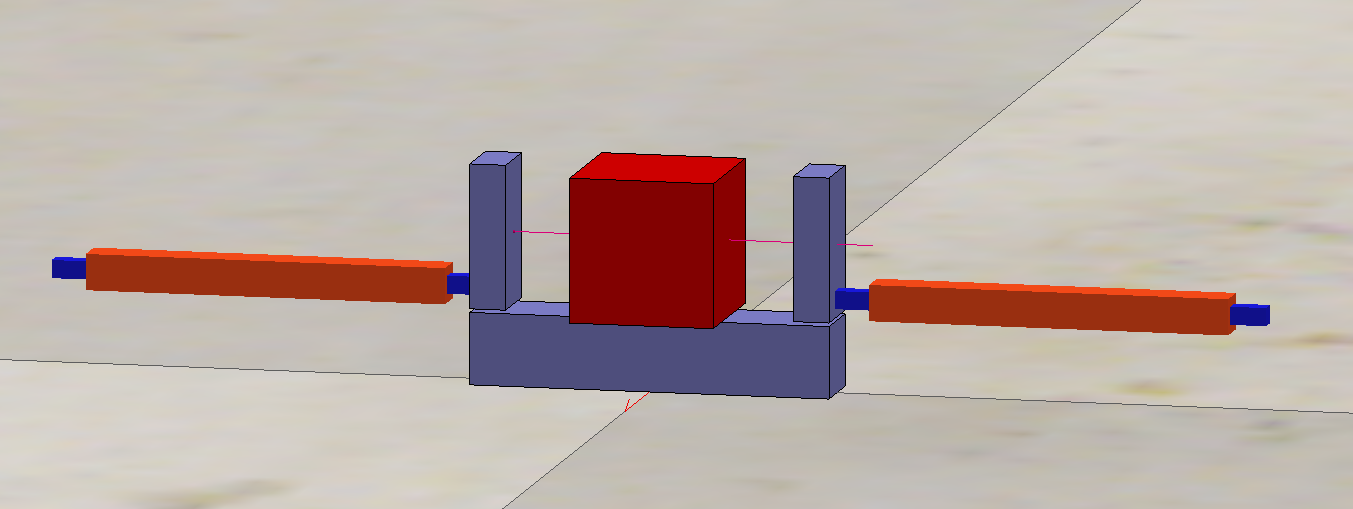
\includegraphics[width=0.75\textwidth]{final_scene.png}
        \caption{Модель схвата}
        \label{pic:L1 gripper}
    \end{figure}

    Напишем скрипт, который будет выполнять следующую последовательность:
    \begin{enumerate}
        \item Схват объекта
        \item Интервал ожидания (5 секунд)
        \item Разжатие объекта
    \end{enumerate}

    Начнём сразу с использования RemoteAPI и выберем Python как язык клиента. Чтобы использовать
    связки с функциями симулятора необходимо из директории симулятора скопировать набор библиотек в свою
    рабочую директорию.

    \sloppy Для обеспечения работы клиента сперва необходимо запустить симуляцию, которая на старте открывает порт
    для внешнего подключения командой \luainline/simRemoteApi.start(19999)/, где аргумент функции есть номер порта.

    На стороне клиента обязательно необходимо открыть подключение с помощью функции \pythoninline/simxStart()/, она
    принимает данные о сервере, как работать с подключением и возвращает ID по которому в дальнейшем нужно отправлять
    все функции. По окончанию работы клиент обязан закрыть подключение функцией \pythoninline/simxFinish()/.

    Одной неприятной особенностью API стало отсутствие привязки к функции \luainline/getSimulationTime()/, поэтому
    пришлось писать небольшую функцию обёртку внутри модели и вызывать её через API. Нежелание использовать
    на клиенте, например, модуль \pythoninline/time/ связано с тем что хотелось использовать именно время симуляции.

    \luafile[firstline=71, lastline=73, frame=single]{../src/gripper_script.lua}
    \pythonfile[firstline=79, lastline=90, frame=single]{../src/main.py}

    Полный код приведён в приложении~\ref{code:remoteAPI}.

    Имея код для клиента довольно легко перенести его на Lua, однако ввиду ограниченных знаний о языке подход будет
    отличаться. Также как и в клиенте напишем раздельные функции, но, поскольку мы используем непотоковые скрипты,
    нельзя явно блокировать процесс циклами \luainline/while/, иначе симуляция зависнет. Поэтому будем использовать
    флаги для обозначения состояния. При этом, чтобы не делать две идентичные модели (одну для API другую для внутренних
    скриптов) мы сможем сделать так, чтобы при запуске симуляции единожды производилась демонстрация работы модели
    используя Lua, после чего можно будет подключиться через API.

    Дополнительно напишем код для преобразования данных с сенсора. Если смотреть на выводимые графики, то видно, что на
    датчике присутствует шум, который скорее всего связан с дискретностью симуляции. Несмотря на то что колебания
    небольшие мы можем написать функцию, которая будет считать скользящее среднее.

    Для этого нам потребуется написать дополнительно следующие функции для суммирования элементов массива, поскольку
    в стандартной библиотеке Lua такая отсутствует.

    \luafile[frame=single, firstline=8, lastline=9]{../src/sensor_script.lua}

    Первая выполняет суммирование произвольного количества аргументов используя рекурсию, вторая "распаковывает" массив
    в отдельные аргументы для этой функции.

    Получим следующие графики
    \begin{figure}[H]
        \centering
        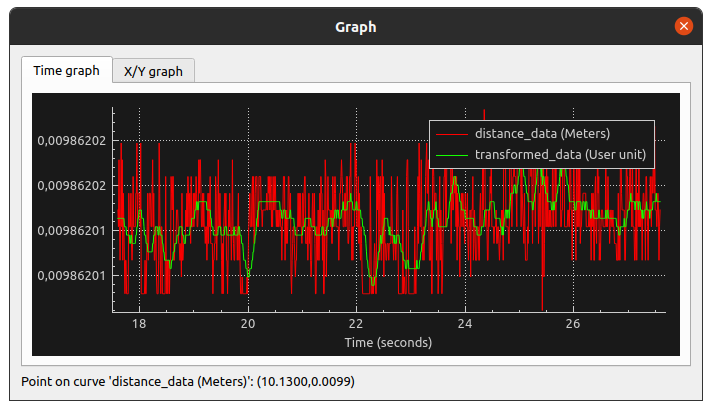
\includegraphics[width=0.75\textwidth]{graph.png}
        \caption{Данные с сенсора от времени}
        \label{pic:graph}
    \end{figure}

    \section*{Вывод}
    В работе была изучена работа с графиками и методы преобразования данных получаемых в процессе симуляции.
    Также исследован список доступных remoteAPI функций для Python и на их основе написан управляющий скрипт.
    Показана идентичность работы симуляции как при работе с клиентом, так и напрямую из скриптов Lua.

    \appendix
    \renewcommand{\thesection}{\Asbuk{section}}
    \section{RemoteAPI скрипт}\label{code:remoteAPI}
    \pythonfile[frame=single]{../src/main.py}

    \section{Скрипт управления схватом на Lua}\label{code:gripper}
    \luafile[frame=single]{../src/gripper_script.lua}

    \section{Скрипт работы с графиком}\label{code:graph}
    \luafile[frame=single]{../src/sensor_script.lua}


\end{document}
